\section[Część analityczno-teoretyczna]{Część analityczno-teoretyczna} % 30% pracy - opis problematyki podjętego tematu w zakresie wykorzystanym w pracy i analizie
    Plazma, powszechnie nazywana czwartym stanem materii, to zbiór
    zjonizowanych cząstek oraz elektronów przejawiających jako grupa globalną
    obojętność elektryczną. Innymi słowy, od gazu plazmy odróżnia fakt, że
    cząstki są zjonizowane, więc oddziałują kolektywnie między sobą na
    odległość, ale ich pola elektryczne wzajemnie się neutralizują na długich
    dystansach.

    Plazmy występują w całym wszechświecie, od materii międzygwiezdnej po
    błyskawice.  Ich istnienie uwarunkowane jest obecnością wysokich energii,
    wystarczających do zjonizowania atomów gazu.

    Fizyka plazmy jest stosunkowo młodą nauką, której rozwój nastąpił dopiero w
    ostatnim stuleciu, zaczynając od badań Langmuira (1928), który
    eksperymentował z jonizowaniem gazów w szklanych rurach zwanych rurami
    Crookesa, służących do generowania promieniowania katodowego, czyli, jak
    wiemy obecnie, strumieni elektronów.

    Globalny wzrost zainteresowania fizyką plazmy na arenie geopolitycznej
    rozpoczął się w latach czterdziestych ubiegłego wieku, gdy uświadomiono sobie,
    że można zastosować ją do przeprowadzania kontrolowanych reakcji syntezy
    jądrowej,
    które mogą mieć zastosowania w energetyce jako następny etap rozwoju po
    reakcjach rozpadu wykorzystywanych w ``klasycznych'' elektrowniach jądrowych.
    Był to jeden z elementów zimnowojennego wyścigu technologicznego między Stanami
    Zjednoczonymi a ZSRR, jak również jeden z projektów mających na celu ponowne
    nawiązanie współpracy naukowej między supermocarstwami po zakończeniu tego
    konfliktu. Obecnie trwają intensywne badania nad tym problemem, których
    dotychczasową kulminacją jest budowany we Francji tokamak ITER i planowany reaktor DEMO.

    Poza tym ogromnym projektem plazmy mają szerokie zastosowania w obecnym
    przemyśle, na przykład:
    \begin{itemize}
        \item metalurgicznym - cięcie metalu przy użyciu łuków plazmowych
        \item elektronicznym i materiałowym - żłobienie powierzchni urządzeń
            półprzewodnikowych, powierzchniowa obróbka materiałów, depozycja
            aktywnych jonów pod powierzchnią czyszczenie powierzchni, depozycja
            cienkich warstw związków chemicznych na powierzchniach (CVD)
        \item kosmicznym - silniki plazmowe, interakcja z rozgrzanym powietrzem
            podczas powtórnego wchodzenia w atmosferę
        \item użytkowym - ekrany telewizorów, oświetlenie (świetlówki)
    \end{itemize}

    Należy też zwrócić uwagę, że ze względu na złożoność układów plazmowych
    pra-komputerowa fizyka miała ogromne problemy z merytorycznymi badaniami
    zachowania plazmy poza wybranymi, mocno uproszczonymi reżimami. Postęp w
    badaniach plazmy, jak sugeruje rozwój technologii kontrolowanej syntezy
    jądrowej, jest silnie skorelowany z
    rozwojem mocy obliczeniowej oraz algorytmów symulacyjnych.\cite{youtube-plasma-algorithm-progress}

    \subsection{Modelowanie i symulacja plazmy}

    Modelowanie zjawisk z zakresu fizyki plazmy jest jednym z bardziej
    złożonych problemów fizyki komputerowej. Głównym, koncepcyjnie, powodem
    uniemożliwiającym zastosowanie prostych metod symulacji znanych z
    newtonowskiej dynamiki molekularnej jest mnogość oddziaływań - każda
    cząstka oddziałuje z każdą inną nawzajem poprzez niepomijalne oddziaływania
    kulombowskie, skalujące się z odległością jak
    $\approx r^{-2}$. Paradoksalnie, na dużych odległościach oddziaływania
    te znoszą się, co rozumie się w plazmie jako \concept{kwaziobojętność} - jednak
    bez uwzględnienia oddziaływań od wszystkich cząstek nie osiągnie się tego
    efektu,

    Z powodu dużej liczby cząstek w układach plazmowych, jedynymi podejściami
    fundamentalnymi (jako opierającymi się na fundamentalnej fizyce) są opisy
    kinetyczne. Wielkością opisującą plazmę jest tu funkcja dystrybucji (zwana
    też funkcją rozkładu) zdefiniowana jako $f_s(\vec{x}, \vec{v}, t) d\vec{x}
    d\vec{v}$ opisująca gęstość rozkładu danej grupy cząstek $s$ plazmy w
    sześciowymiarowej przestrzeni fazowej (po trzy wymiary na położenia oraz
    prędkości). Ewolucja czasowa funkcji rozkładu dokonuje się poprzez
    rozwiązanie wariantu równania Boltzmanna zwanego równaniem Vlasova,
    które sprzęga gęstości ładunku i prądu otrzymywane z funkcji dystrybucji
    z równaniami Maxwella na ewolucję pola elektromagnetycznego.

    Dla przypadku plazmy złożonej z elektronów i jednego rodzaju jonów o ładunku $Z_i$:

    \begin{align}
    \frac{\partial f_e}{\partial t} + \vec {v}_e\cdot\nabla f_e &- e\left(\vec {E}+\vec {v_e}\times\vec {B}\right)\cdot\frac{\partial f_e}{\partial\vec {p}} = 0
    \label{eqn:vlasov-electrons}\\
    \frac{\partial f_i}{\partial t} + \vec {v}_i\cdot\nabla f_i &+ Z_i e\left(\vec {E}+\vec {v_i}\times\vec {B}\right)\cdot\frac{\partial f_i}{\partial\vec {p}} = 0
    \label{eqn:vlasov-ions}\\
    \nabla\times\vec {B} &=\mu_0 \left(\vec{j}+\epsilon_0 \frac{\partial \vec {E}}{\partial t}\right)
    \label{eqn:maxwell-B-rotation}\\
    \nabla\times\vec {E} &=-\frac{\partial\vec {B}}{\partial t}
    \label{eqn:maxwell-E-rotation}\\
    \nabla\cdot\vec {E}  &=\rho / \epsilon_0
    \label{eqn:maxwell-E-div}\\
    \nabla\cdot\vec {B}  &=0
    \label{eqn:maxwell-B-div}
    \end{align}

    Równanie Vlasova może zostać rozszerzone do równania Fokkera-Plancka uwzględniającego
    bezpośrednie kolizje międzycząsteczkowe.

    W praktyce równanie Vlasova jest trudne do rozwiązania poza trywialnymi
    przypadkami o ułatwiających problem symetriach.  Jednym z powodów tej
    trudności jest konieczność uzyskania dobrej rozdzielczości prędkości przy
    jednoczesnym zachowaniu zakresów obejmujących prędkości relatywistyczne.
    Jako równanie różniczkowe cząstkowe, równanie Vlasova jest rozwiązywane na
    dyskretnych siatkach, należy zauważyć zaś, że skalowanie
    liczby punktów na siatce tego typu jest proporcjonalne do $N_r^3 N_v^3$,
    gdzie $N_r$ to liczba punktów przestrzennych, zaś $N_v$ to liczba punktów
    na siatce prędkości. Jest to więc często niepraktyczne obliczeniowo,
    między innymi ze względu na istotne w plazmach fuzyjnych zjawisko
    ``uciekających elektronów'' o relatywistycznych prędkościach.

    W modelowaniu komputerowym plazmy stosuje się trzy główne koncepcyjne podejścia:
    \begin{enumerate}
        \item modele kinetyczne rozwiązujące bezpośrednio równania typu Vlasova
            na dyskretnych siatkach
        \item modele płynowe oparte na ciągłym opisie plazmy poprzez
            uśrednienie po dystrybucji wielkości termodynamicznych, co daje
            modele takie jak magnetohydrodynamikę. Jest to wciąż układ równań
            różniczkowych cząstkowych, lecz na mniej wymiarowej siatce.
            Niestety, nie nadają się one do badań plazmy daleko od równowagi z
            powodu czynionych przy nich założeń takich jak maxwellowski rozkład
            prędkości. Znajdują za to szerokie zastosowanie w astronomii.
        \item modele dyskretne oparte na samplowaniu dystrybucji plazmy przy
            użyciu dyskretnych cząstek, pozwalające w prosty sposób uzyskać
            dobre przybliżenie faktycznego ruchu cząstek w plazmie i prądów
            generowanych tym ruchem. Pozwalają na wizualizację efektów działań
            pól, ale potrafią być mało wydajne do modelowania efektów kolektywnych.
            \todo[inline]{czy na pewno należy rozróżniać kinetyczne i dyskretne?}
    \end{enumerate}

    Istnieje bardzo popularna klasa modeli łączących cechy kategorii pierwszej i trzeciej.
    Są to tak zwane modele Particle-in-cell.

    \subsection{Modele Particle-in-cell}

    Idea modelu \concept{particle-in-cell} (dalej nazywanego \concept{PIC}) jest wyjątkowo
    prosta i opiera się na idei przyspieszenia najbardziej złożonego obliczeniowo
    kroku symulacji dynamiki molekularnej, czyli obliczania sił
    międzycząsteczkowych.  Cząstki poruszają się w ciągłej, Lagrange'owskiej
    przestrzeni.  Ich ruch wykorzystywany jest do zebrania informacji dotyczącej
    gęstości ładunku i prądu na dyskretną, Eulerowską siatkę. Na siatce rozwiązane
    są (jako równania różniczkowe cząstkowe) równania Maxwella, dzięki którym
    otrzymuje się pola elektryczne i magnetyczne, które z powrotem są przekazane do
    położeń cząstek.  Obliczeniowo, uwzględniając koszty odpowiednich interpolacji,
    pozwala to zredukować złożoność kroku obliczenia sił międzycząsteczkowych do złożoności $O(n)$ z $O(n^2)$.
    Oczywiście, jest to okupione zależnością złożoności od liczby punktów na siatce $m$, lecz jako że $m << n$,
    jest to akceptowalne i korzystne.

    \subsubsection{Pętla obliczeniowa PIC}
    Obliczeniowo algorytm particle-in-cell składa się z czterech elementów
    powtarzających się cyklicznie:
    \begin{itemize}
        \item Zbierz (\english{Gather})\\
    Depozycja ładunku oraz prądu z położeń cząstek do lokacji na dyskretnej
    siatce poprzez interpolację, co pozwala na sprawne rozwiązanie na tej
    siatce równań Maxwella jako układu różnicowych równań cząstkowych zamiast
    obliczania skalujących się kwadratowo w liczbie cząstek oddziaływań
    kulombowskich między nimi.  W naszym elektromagnetycznym przypadku bardziej
    istotną jest depozycja prądu na siatkę, co szerzej tłumaczy następny
    fragment.
    \item Rozwiąż (\english{Solve})\\
    Sprawne rozwiązanie równań Maxwella na dyskretnej, Eulerowskiej siatce.
    Znalezienie pól elektrycznego i magnetycznego na podstawie gęstości ładunku
    i prądu na siatce.  Istnieją dwie główne szkoły rozwiązywania tych równań:
    metody globalne i lokalne. Metody globalne wykorzystują zazwyczaj równania
    dywergencyjne (prawa Gaussa)\ref{eqn:maxwell-E-div}\ref{eqn:maxwell-B-div}
    rozwiązywane iteracyjnie (metodami takimi jak Gaussa-Seidela lub gradientów
    sprzężonych)
     lub spektralnie, przy użyciu transformat Fouriera lub Hankela~\cite{fbpic}.
     Metody lokalne z kolei
    wykorzystują równania rotacyjne (prawa Ampera-Maxwella\ref{eqn:maxwell-E-rotation}
    oraz Faradaya\ref{eqn:maxwell-B-rotation}):

    Metody globalne nadają się do modeli elektrostatycznych,
    nierelatywistycznych.  Metody lokalne pozwalają na ograniczenie szybkości
    propagacji zaburzeń do prędkości światła, co przybliża metodę numeryczną do
    fizyki zachodzącej w rzeczywistym układzie tego typu.
    \item Rozprosz (\english{Scatter}) \\
    Interpolacja pól z siatki do lokacji cząstek, co pozwala określić siły
    elektromagnetyczne działające na cząstki.  Należy przy tym zauważyć, że
    jako że interpolacja sił wymaga jedynie lokalnej informacji co do pól
    elektromagnetycznych w okolicy cząstki, ta część algorytmu sprawia, że
    algorytmy Particle-in-cell doskonale nadają się do zrównoleglenia (problem
    jest w bardzo dobrym przybliżeniu ``trywialnie paralelizowalny''). Z tego
    powodu algorytmy Particle-in-cell nadają się doskonale do wykorzystania
    rosnącej mocy kart graficznych i architektur GPGPU.
    \item Porusz (\english{Push}) \\
    iteracja równań ruchu cząstek
    \begin{equation}
        d \vec{p}/dt = \vec{F} = q (\vec{E} + \vec{v} \times \vec{B})
        \label{eq-of-motion}
    \end{equation}
    na podstawie ich prędkości (aktualizacja położeń) oraz działających na nie
    sił elektromagnetycznych (aktualizacja prędkości). Należy zauważyć, że
    modele PIC nie modelują bezpośrednich kolizji między cząstkami. Kolizje
    mogą jednak zostać dodane niebezpośrednio, na przykład poprzez metody Monte
    Carlo.

    Jako że każda cząstka, zakładając znane pola elektromagnetyczne w jej
    położeniu, porusza się niezależnie, jest to kolejny fragment doskonale
    nadający się do zrównoleglenia.
    \end{itemize}
    \subsubsection{Makrocząstki}
    Należy zauważyć, że obecnie nie jest jeszcze możliwe dokładne odwzorowanie
    dynamiki układów plazmowych w sensie interakcji między poszczególnymi
    cząstkami ze względu na liczbę cząstek rzędu liczby Avogadro $\approx
    10^{23}$.  W tym kontekście bardzo szczęśliwym jest fakt, że wszystkie
    istotne wielkości zależą nie od ładunku ani masy, ale od stosunku $q/m$. W
    praktyce stosuje się więc \emph{makrocząstki}, obdarzone ładunkiem i masą
    będące wielokrotnościami tych wielkości dla cząstek występujących w naturze
    (jak jony i elektrony, pozwalając jednocześnie zachować gęstości cząstek i
    ładunku zbliżone do rzeczywistych.

    Makrocząstki posiadają też kształt, który wyraża się w symulacji poprzez
    interpolację wielkości fizycznych znanych na siatce Eulera do położeń
    cząstek i odwrotnie. Matematycznie jest to opisane poprzez funkcję kształtu.
    Najprostszą jednowymiarową funkcją kształtu (oznaczaną $S_0$) jest funkcja
    ``cylindrowa'', która oznacza jednorodny rozkład gęstości cząstki w zakresie
    szerokości równym długości jednej komórki.
    
    Inne funkcje kształtu tworzy się poprzez kolejne sploty funkcji podstawowej,
    co obrazuje rysunek\ref{fig:shapefunctions}. Funkcja $S_1$ (trójkątna,
    skupiona na środku) jest tradycyjną funkcją ksztąłtu wykorzystywaną
    historycznie w większości zastosowań modelu PIC.


    \begin{figure}[h!]
      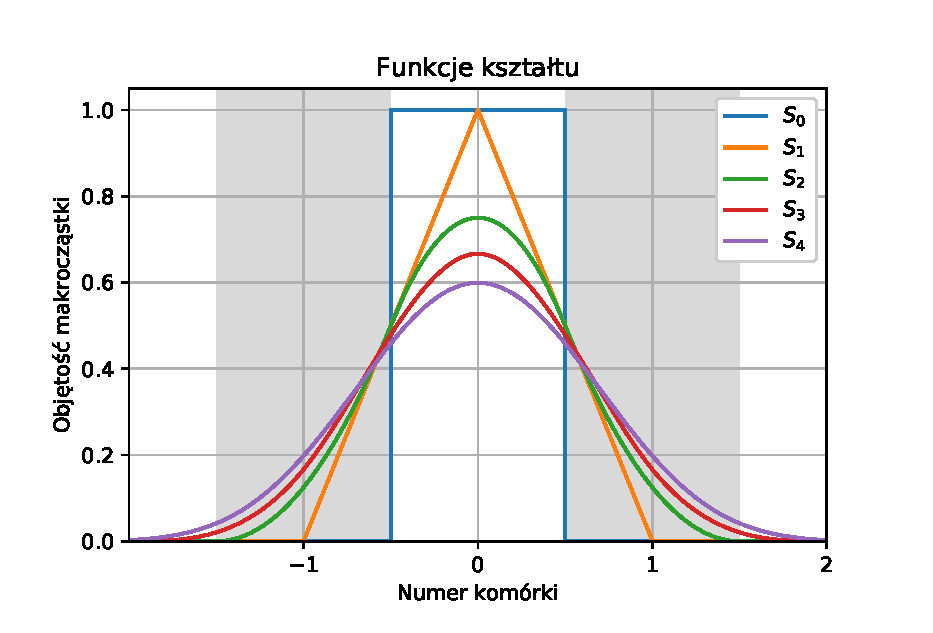
\includegraphics{Images/shapefunctions}
      \label{fig:shapefunctions}
      \caption{Typowe funkcje kształtu dla makrocząstki}
    \end{figure}

    W symulacjach elektromagnetycznych zazwyczaj (``tradycyjnie'') stosuje się
    gęstości cząstek (rzeczywistych) rzędu jednej dziesiątej bądź setnej
    gęstości krytycznej plazmy $n_c$ (wyrażaną wzorem~\ref{eqn:critical-density}),
    która oznacza taką koncentrację
    elektronów, przy której fala laserowa zaczyna być tłumiona zamiast być
    przepuszczaną przez plazmę.\cite{chen}

    \begin{equation}
        n_c = m_e \varepsilon_0 * {(\frac{2 \pi c}{e \lambda})}^2
        \label{eqn:critical-density}
    \end{equation}
    gdzie $m_e$ to masa spoczynkowa elektronu, $\varepsilon_0$ to przenikalność
    elektryczna próżni, $c$ to prędkość światła w
    próżni, $e$ to ładunek elementarny, zaś $\lambda$ to długość fali.

    Gęstość takiej makrocząstki, oznaczana $n_{pic}$, oznacza innymi słowy
    liczbę rzeczywistych cząstek, jakie reprezentuje sobą jedna makrocząstka.

    \subsection{Problem testowy}

    Głównym problemem testowym, jakiego używamy do przetestowania dokładności i
    wydajności działania algorytmu jest interakcja impulsu laserowego z tarczą
    składającą się ze zjonizowanego wodoru i elektronów.

    Układ ten modelowany jest jako jednowymiarowy. Jest to tak zwany w
    literaturze model 1D-3D.  O ile położenia cząstek są jednowymiarowe ze
    względu na znaczną symetrię cylindryczną układu, cząstki mają prędkości w
    pełnych trzech wymiarach. Jest to konieczne ze względu na oddziaływania
    cząstek z polem elektromagnetycznym propagującym się wzdłuż osi układu
    i możliwość dowolnego dobrania kierunku polaryzacji promieniowania
    laserowego w symulacji.

    Układ ten jest silnie zbliżony do rzeczywistych eksperymentów prowadzonych
    w Instytucie Fizyki Plazmy i Laserowej Mikrosyntezy.  \todo[inline]{Tu bym
    chciał prosić o weryfikację.}

    \subsection{Python}
    Python jest wysokopoziomowym, interpretowanym językiem programowania,
    którego atutami są
    \begin{itemize}
    \item otwartość i dostępność
    \item szybkie prototypowanie dzięki wbudowanemu środowisku \english{REPL}, rozszerzalnemu przez pakiet IPython\cite{ipython}
    \item możliwość łatwej integracji z innymi, niskopoziomowymi językami, między innymi C.
    \item łatwy dostęp do szerokiej gamy darmowych blibliotek na licencji \english{open source}, w tym naukowych i numerycznych
    \item wieloplatformowość, łatwość uruchomienia tych samych programów na wielu różnych maszynach
    \end{itemize}

    Python znajduje szerokie zastosowania w analizie danych i uczeniu maszynowym
    (zwłaszcza w astronomii\cite{astropy}). W zakresie symulacji w ostatnich czasach powstały
    kody skalujące się nawet w zakres superkomputerów, na przykład w mechanice
    płynów.  Nie można tu nie wspomnieć o utworzonym niedawno hydrodynamicznym kodzie
    PyFR, łączącym szybkie obliczenia w CUDA, OpenCL oraz OpenMP z wysokopoziomowością Pythona. Uruchomiono go na klastrze Piz Daint
    i udowodniono jego skalowanie (\english{weak scaling}) do 2000 kart NVIDIA K20X i 1.3 stabilnych petaflopów na sekundę.
    \cite{pyfr}\cite{pyfr-euroscipy}


    Atutem Pythona w wysokowydajnych obliczeniach jest łatwość użycia w
    nim zewnętrznych bibliotek napisanych na przykład w C lub Fortranie, co
    pozwala na osiągnięcie podobnych rezultatów wydajnościowych jak dla kodów
    napisanych w językach niskopoziomowych bez faktycznej pracy z tymi
    językami.

    Istotną zaletą Pythona, o której nie można nie wspomnieć, jest inherentna
    otwartość wśród użytkowników tego języka. Znacząca część projektów tworzonych w
    tym języku jest udostępnianych za darmo jako projekty \english{open source},
    internecie na platformach takich jak GitHub, GitLab i Bitbucket, co znacząco
    ułatwia kolaborację i wspólne ich tworzenie przez społeczność.  Jest to obszar,
    którego techniki wydają się być równie korzystne w społeczności naukowej, jak pokazują
    wyniki grup badawczych \cite{labarba}. %TODO011 reference labarba

    \subsubsection{Numpy}
    \code{numpy}\cite{numpy} to biblioteka umożliwiająca wykonywanie złożonych obliczeń na
    n-wymiarowych macierzach bądź tablicach, utworzona w celu umożlwiienia
    zastąpienia operacjami wektorowymi iteracji po tablicach, powszechnie
    stosowanych w metodach numerycznych i będących znanym słabym punktem
    Pythona.

    Pod zewnętrzną powłoką zawiera odwołania do znanych, wypróbowanych i
    sprawdzonych w numeryce modułów \code{LAPACK}, \code{BLAS} napisanych w
    szybkich, niskopoziomowych językach C oraz \code{FORTRAN}.  Jest to
    \emph{de facto} standard większości obliczeń numerycznych w Pythonie.

    Należy zauważyć, że operacje matematyczne w wersji \code{numpy} zawartej
    w dystrybucji Anaconda są automatycznie
    zrównoleglane tam, gdzie pozwala na to
        niezależność obliczeń dzięki dołączonym bibliotekom Intel Math Kernel Library.\cite{intel-mkl} 

    Numpy jest oprogramowaniem otwartym, udostępnianym na licencji BSD.


    \subsubsection{scipy}
    Kolejną podstawową biblioteką w numerycznym Pythonie jest \code{scipy},
    biblioteka zawierająca wydajne gotowe implementacje wielu powszechnych algorytmów
    numerycznych służących między innymi całkowaniu, optymalizacji funkcji rzeczywistych,
    uczeniu maszynowemu, algebrze liniowej czy transformatom Fouriera.

    \subsubsection{Numba}
    \code{numba} to biblioteka służąca do kompilacji just-in-time wysokopoziomowego
    kodu Pythona do kodu niskopoziomowego przy pierwszym uruchomieniu programu. W
    wielu przypadkach pozwala na osiągnięcie kodem napisanym w czystym Pythonie
    wydajności marginalnie niższej bądź nawet równej do analogicznego programu w C
    bądź Fortranie. \cite{numba}

    Jednocześnie należy zaznaczyć prostotę jej użycia. W wielu przypadkach wystarczy
    dodać do funkcji dekorator \code{@numba.jit}:


    \todo[inline]{fragment kodu. @jit przed kodem} % TODO003 numba code part


    Istniejącym od niedawna kodem symulacyjnym implementującym tą metodę jest FBPIC\cite{fbpic}.


    \subsubsection{HDF5}
    HDF5 jest wysokowydajnym formatem plikow służącym przechowywaniu danych
    liczbowych w drzewiastej, skompresowanej strukturze danych, razem z
    równoległym, wielowątkowym zapisem tych danych.  W Pythonie implementuje go
    biblioteka h5py\cite{h5py}.

    W bieżącej pracy wykorzystuje się go do przechowywania danych liczbowych
    dotyczących przebiegu symulacji, pozwalających na ich dalsze przetwarzanie
    i analizę poprzez wizualizację.

    \subsubsection{matplotlib}
    Do wizualizacji danych z symulacji (oraz tworzenia schematów w sekcji
    teoretycznej niniejszej pracy) użyto własnoręcznie napisanych skryptów w
    uniwersalnej bibliotece graficznej \code{matplotlib}\cite{matplotlib}.
    \code{matplotlib} zapewnia wsparcie zarówno dla grafik statycznych w różnych układach
    współrzędnych (w tym 3D), jak również dla dynamicznie generowanych animacji
    przedstawiających przebiegi czasowe symulacji.

    \subsubsection{py.test}
    Przy pracy nad kodem użyto frameworku testowego \code{py.test} \cite{pytest}.
    Tworzenie testów jest trywialne:

    \begin{lstlisting}[language=Python, caption=Podstawowy przykład testu w pliku \code{func.py}]
    def f(x):
        return 3*x

    def test_f():
        assert f(4) == 12
    \end{lstlisting}

    Uruchamianie zaś:

    \begin{lstlisting}[language=Bash]
        pytest func.py
    \end{lstlisting}

    Należy zaznaczyć, że w numeryce, gdzie błędne działanie programu nie
    objawia się zazwyczaj formalnym błędem, a jedynie błędnymi
    wynikami, dobrze zautomatyzowane testy jednostkowe potrafią zaoszczędzić
    bardzo dużo czasu na debugowaniu poprzez automatyzację uruchamiania
    kolejnych partii kodu i lokalizację błędnie działających części algorytmu.
    Dobrze napisane testy są praktycznie koniecznością w dzisiejszych czasach,
    zaś każdy nowo powstały projekt numeryczno-symulacyjny powinien je
    wykorzystywać, najlepiej do weryfikacji każdej części algorytmu z osobna.

    Dobrym przykładem skutecznego testu jednostkowego jest porównanie energii kinetycznej
    elektronu o znanej prędkości z wartością tablicową, zawarte jako test w pliku
    \code{pythonpic/tests/test\_species.py}.

    \code{py.test} jest oprogramowaniem otwartym, dostępnym na licencji MIT.

    \subsubsection{Travis CI}
    Nieocenionym narzędziem w pracy nad kodem był system ciągłej integracji
    (\emph{continuous integration}) Travis CI \cite{travisci}
    dostępny za
    darmo dla projektów open-source. Travis pobiera aktualne wersje kodu przy
    każdej aktualizacji wersji dostępnej na serwerze GitHub i uruchamia testy,
    zwracając komunikat o ewentualnym niepowodzeniu i pozwalając na jednoczesne
    uruchamianie bieżących, intensywnych symulacji przy jednoczesnym
    weryfikowaniu w chmurze poprawności działania lżejszych, acz wciąż intensywnych
    symulacji testowych i testów algorytmicznych.

    \subsubsection{snakeviz}

    W optymalizacji przydatny okazał się program \code{snakeviz}\cite{snakeviz} dostępny na
    GitHubie i pozwalający na wizualizację wyników z profilowania
    symulacji. Pozwala w wygodny sposób zbadać, które fragmenty kodu najbardziej
    spowalniają symulację, które są najlepszymi kandydatami do optymalizacji, oraz
    jak skuteczne (bądź nieskuteczne) okazują się próby polepszenia ich wydajności.
    Działanie programu ilustruje rysunek~\ref{fig:snakeviz}.
    \begin{figure}[h!]
      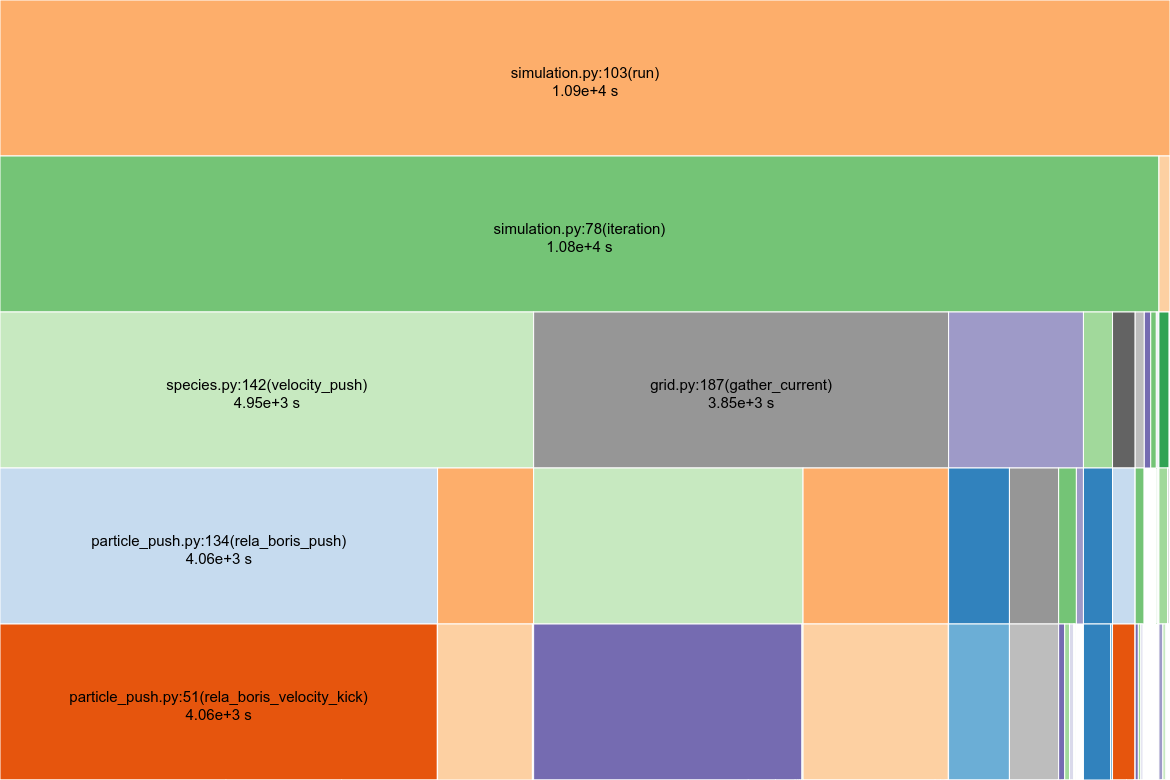
\includegraphics[width=\textwidth]{Images/snakeviz}
      \caption{Wizualizacja szybkości działania poszczególnych fragmentów kodu
        wygenerowana programem snakeviz.}
      \label{fig:snakeviz}
    \end{figure}
